\head{Ноябрь}{Теоретический Листок. Комбинаторика.}

\begin{figure}[h!]
\begin{minipage}{0.45\linewidth}~\hfill
    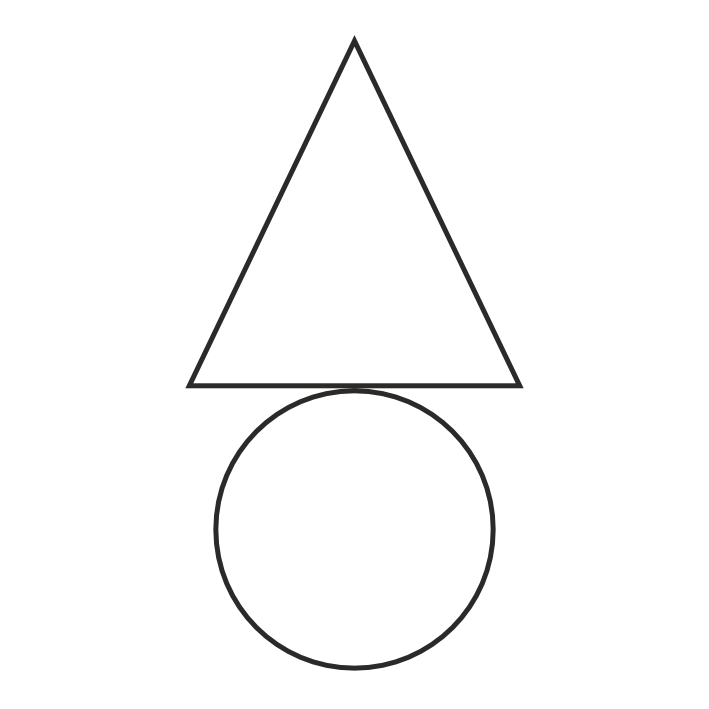
\includegraphics[scale=0.3]{./img/tr}
	\hfill~
\end{minipage}
\begin{minipage}{0.5\linewidth}\setlength{\parindent}{1.5em}
\epigraph{\textit{Раз, два, три, четыре, пять, шесть, семь, восемь, девять, десять -
		можно все пересчитать, или же измерить, взвесить...
}}{Считалка из учебника математики для 1 класса}
\end{minipage}
\end{figure}

\begin{figure}[h!]
\begin{minipage}{0.84\linewidth}\setlength{\parindent}{1.5em}
Пусть у нас есть три треугольника и два круга. Мы хотим составить фигурку такую как на рисунке сверху. Сколькими способами мы можем это сделать? Понятно, что выбор круга и выбор треугольника никак не зависят друг от друга. С любым из кругов можно выбрать любой из треугольников. Возможные комбинации приведены на рисунке справа. Итого 6 вариантов. 
\end{minipage}
\begin{minipage}{0.15\linewidth}
    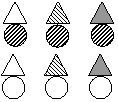
\includegraphics[width=0.9\columnwidth]{./img/tre}
\end{minipage}
\end{figure}

\begin{figure}[h!]
\begin{minipage}{0.15\linewidth}
    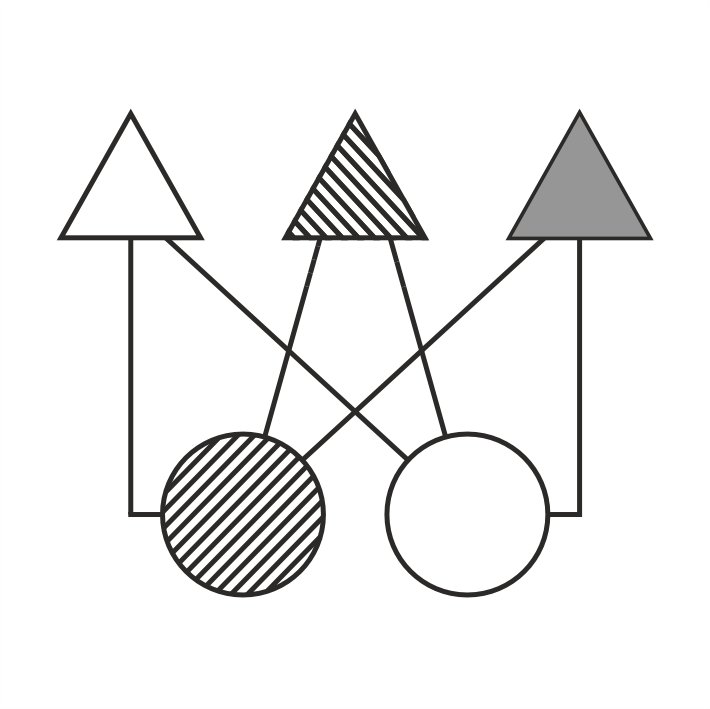
\includegraphics[width=0.9\columnwidth]{./img/komb}
\end{minipage}
\begin{minipage}{0.84\linewidth}\setlength{\parindent}{1.5em}
Этот же факт можно проиллюстрировать по-другому - см. рисунок слева. Те фигурки, которые можно поставить в пару, соединены линией. Сколько линий, столько и вариантов. И наконец третья иллюстрация - треугольник мы можем выбрать тремя способами, а круг - двумя, следовательно, всего $3 \times 2 = 6$ вариантов.\\ Итак, окончательный \underline{\textit{ответ:}} 6 способов.
\end{minipage}
\end{figure}

\begin{figure}[!h]
\begin{minipage}{0.84\linewidth}\setlength{\parindent}{1.5em}
\begin{thm}
	Из города A в город B ведут 3 дороги, а из города B в город C - 2 дороги. Сколькими способами можно проехать из A в C? 
\end{thm}
\begin{prf} Понятно, что выбор дороги между А и В никак не связан с выбором дороги между В и С. Поэтому из А в В мы можем доехать тремя способами, а из В в С - двумя способами. Поэтому всего способов - $3 \times 2 = 6$. \underline{\textit{Ответ:}} 6 способов.\footnotemark
\end{prf}
\end{minipage}
\begin{minipage}{0.15\linewidth}
    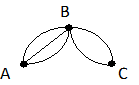
\includegraphics[width=0.9\columnwidth]{./img/ways}
\end{minipage}
\end{figure}
\footnotetext{Заметим, что эта задача полностью аналогична предыдущей задача про выбор треугольников и кружков: можно, например, считать, что дороги из А в В помечены одним из треугольников и выбор дороги означает выбор треугольника, а дороги из В в С помечены кругами и выбор дороги означает выбор одного из двух кругов.}

\begin{figure}[!h]
\begin{minipage}{0.2\linewidth}
    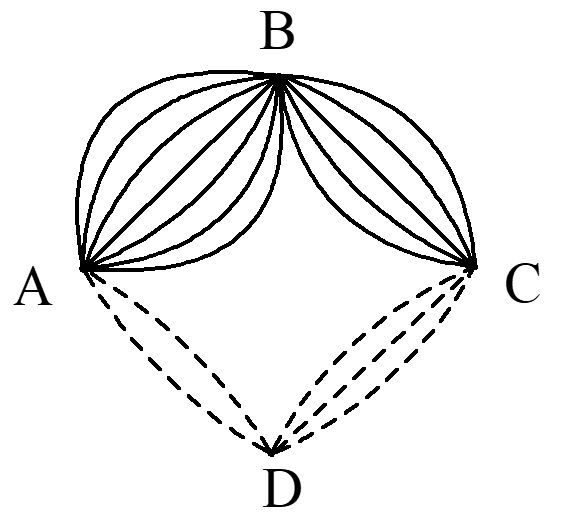
\includegraphics[width=0.9\columnwidth]{./img/ways2}
\end{minipage}
\begin{minipage}{0.79\linewidth}\setlength{\parindent}{1.5em}
\begin{ex}\label{u14}
	а) Из города А в город В ведут 7 дорог, а из города В в город С - 5 дороги. Сколькими способами можно проехать из А в С?
	\\	
	б) Построили новый город D и из него 2 дороги ведут в А и 3 в С. Сколькими способами теперь можно проехать из А в С?
\end{ex}
\end{minipage}
\end{figure}

\begin{ex}\label{u15}
	Кощей Бессмертный, желая сделать Бабе Яге подарок на Новый Год, приобрел кучу метелок трех сортов, ступы 5 сортов и головные платки 7 расцветок. Он хочет каждый Новый Год дарить Яге 1 метлу, 1 ступу и 1 платок, но так, чтобы ни один год наборы подарков не совпадали. На сколько лет ему хватит приобретенных товаров?\footnote{Считайте, что количество приобретенных предметов сколь угодно велико.}
\end{ex}

\fbox{
\begin{minipage}{0.93\linewidth}\centering	
\textbf{Основное правило комбинаторики.}

\textit{Если какое-то действие можно разбить на два, и первое из них можно осуществить $n$ способами, а второе - $m$ способами, то все действие можно осуществить $ m\times n$ способами.}
\end{minipage}
}

\begin{ex}\label{u16}
	Переформулируйте предыдущее упражнение как задачу про дороги. 
\end{ex}

\begin{thm}
	Монету бросают трижды. Сколько различных последовательностей орлов и решек можно получить? 
\end{thm}

\begin{prf}
	Для каждого из трех бросков имеется только два варианта: «орел» или «решка». Результат каждого броска не зависит друг от друга. Поэтому вариантов последовательностей восемь. \footnote{При желании их все можно выписать}\\ \underline{\textit{Ответ:}} 8 последовательностей.
\end{prf}

\begin{ex}\label{u17}
	А если в предыдущей задаче бросать монету сто раз?
\end{ex}

\begin{ex}\label{u18}
	Переформулируйте предыдущую задачу как задачу про дороги. 
\end{ex}

\begin{thm}Назовем число симпатичным, если в его записи встречаются только нечетные цифры. Сколько существует симпатичных пятизначных чисел?
\end{thm}

\begin{prf}
	Если цифры могут быть только нечетные, то вариантов для каждой позиции пять (1, 3, 5, 7 и 9). Выбор каждой цифры независим. Поэтому вариантов $5^5$.\\ \textit{\underline{Ответ:}} Всего $5^5$ симпатичных чисел.
\end{prf}

\begin{thm}
	Сколько всего пятизначных чисел, которые не симпатичные, но и не неинтересные?
\end{thm}

\begin{prf}
	Число симпатичное, если в его записи встречаются только нечетные цифры, число неинтересное, если в его записи присутствуют только четные цифры. Поскольку каждая цифра либо четная, либо нечетная, то число не может быть одновременно симпатичным и неинтересным. Поэтому, если мы из общего количества пятизначных чисел вычтем количество симпатичных и количество неинтересных, то получим искомое.
	Всего пятизначных чисел 90000. Это можно сосчитать двумя способами:\\ 1) всего натуральных чисел от 1 до 99999 (последнее пятизначное число) -- 99999, однако числа от 1 до 9999 (всего 9999 штук) -- не более, чем четырехзначные;\\ 2) в пятизначном числе на первом месте может стоять любя цифра кроме 0, поэтому вариантов -- 9, а на каждом их оставшихся четырех местах -- любая из 10 цифр, поскольку выбор каждой цифры осуществляется независимо, то всего $9\times10^4 = 90000$ вариантов.\\
	Сосчитаем теперь количество симпатичных чисел. Поскольку имеется пять нечетных цифр - $1, 3, 5, 7, 9$ и любая из них может стоять на любом из пяти мест, то всего симпатичных пятизначных чисел $5^5$.
	Неинтересные числа: имеется также пять четных цифр - $0, 2, 4, 6, 8$, но на первом месте может стоять лишь одна из четырех (число не может начинаться с нуля). Поэтому вариантов неинтересных пятизначных чисел $4\times 5^4$.
	Итак, искомое количество равно\\ $ 90000 - 5^5 - 4\times 5^4 = 90000 - 5^4 = 90000 - 9\times625 = 90625 - 6250 = 83275 $
\end{prf}

Во многих комбинаторных задачах для записи результата потребуется понятие \textit{факториала}:

\fbox{
\begin{minipage}{0.93\linewidth}\centering	
\textit{Факториалом натурального числа $N$ называется произведение всех целых чисел от 1 до $N$: $N!=1\times 2\times 3\times 4 \times\dots \times (N-1)\times N$ (читается “эн факториал”)}
\end{minipage}
}

Хотя факториал определен только для натуральных $N$, удобно ввести понятие $0!$ - будем считать его равным единице.

\begin{ex}\label{u19}
	Чему равно а) $19!\times20$;~~  б) $6!\times56$;~~  в) $N!\times(N + 1)$?
\end{ex}

\begin{ex}\label{u20}
	Чему равно а) $\dfrac{101!}{99!}$;~~  б) $\dfrac{N!}{(N-1)!}$;  
\end{ex}

\begin{thm}
	Сколькими способами можно расположить а) 11 человек в шеренгу;~~ б) 11 разноцветных бусин по кругу?~~ в) Укажите отличия между пунктами а) и б).  
\end{thm}

В предыдущей задаче рассматривается число способов, которыми можно расставить в шеренгу 11 человек. Такое расположение называется \textit{перестановкой}. Таким образом, в этой задаче ищется число перестановок 11 человек. Число перестановок из $N$ предметов обозначается $P_N$.

\begin{thm}\label{3.6}
	Выведите формулу для $P_N$ .
\end{thm}